\usetikzlibrary{arrows.meta,chains}

\begin{frame}\frametitle{files in building C programs [dynamic linking]}
    % FIXME: alt text
\begin{tikzpicture}
\tikzset{
    file/.style={font=\small,draw,align=center},
    file C/.style={file},
    file H/.style={file},
    file system/.style={file,dotted,fill=blue!10},
    file S/.style={file},
    file O/.style={file},
    produce main/.style={draw,very thick,-Latex},
    compile/.style={alt={<2>{red!30!orange}},alt=<3>{invisible}},
    compile alt/.style={alt={<2>{red!30!magenta}},alt=<3>{invisible}},
    compile result/.style={alt=<2>{fill=orange!10,ultra thick,overlay}},
    compile result alt/.style={alt=<2>{fill=magenta!10,ultra thick}},
    compile to S/.style={alt={<3>{red!50!orange}}},
    compile to S alt/.style={alt={<3>{red!50!magenta}}},
    compile to S result/.style={alt=<3>{fill=orange!10,ultra thick,overlay}},
    compile to S result alt/.style={alt=<3>{fill=magenta!10,ultra thick}},
    produce minor/.style={draw,thick},
    linker/.style={alt={<4>{red,very thick}}},
    linker result/.style={alt=<4>{fill=red!10,ultra thick}},
    loader/.style={alt={<5>{red,very thick}}},
}
\begin{scope}[every node/.style={on chain},start chain=going right,node distance=.5cm]
\node[file C] (main c) {main.c};
\node[file H] (main h) {main.h};
\node[file H] (extra h) {extra.h};
\node[file system] (stdio h) {stdio.h};
\node[file C] (extra c){extra.c};
\end{scope}
\node[file O,anchor=north,compile result] (main o) at ([yshift=-2cm]main c.south) {main.o};
\draw[produce main,compile] (main c) -- (main o);
\foreach \nm in {main h,extra h,stdio h} {
    \draw[produce minor,compile] ([xshift=-1mm]\nm.south) |- ([yshift=.5cm]main o.north) -- (main o.north);
}
\node[file O,anchor=north,compile result alt] (extra o) at ([yshift=-2cm]extra c.south) {extra.o};
\draw[produce main,compile alt] (extra c) -- (extra o);
\foreach \nm in {extra h,stdio h} {
    \draw[produce minor,compile alt] ([xshift=1mm]\nm.south) |- ([yshift=1cm]extra o.north) -- (extra o.north);
}
\node[file,linker result] (program) at ([xshift=3cm,yshift=-2cm]main o.south) { program \\ \scriptsize executable };
\node[anchor=west, file system] (compiler o) at ([xshift=1cm]extra o.east) { (system files) };
\foreach \nm in {main o,extra o,compiler o} {
    \draw[produce main,linker] ([xshift=1mm]\nm.south) |- ([yshift=1cm]program.north) -- (program.north);
}
\node[file system,anchor=west] (libc so) at ([xshift=5cm]program.east) {
    libc.so
};
\draw[dotted,thick,loader] (program) -- (libc so) node[fill=white,midway,font=\small] {loads at runtime};

\coordinate (annotate) at ([xshift=-2cm,yshift=-0.2cm]program.south west);
\tikzset{
    action/.style={at={(annotate)},anchor=north west,align=left},
}
\begin{visibleenv}<2>
    \node[action] {
        \texttt{clang -c main.c} \\
        \texttt{clang -c extra.c} 
    };
\end{visibleenv}
\begin{visibleenv}<3>
    \node[file S,anchor=south,compile to S result] (main S) at ([yshift=.5cm]main o.north) {
        main.s
    };
    \draw[produce main,compile to S] (main c) |- ([yshift=.5cm]main S.north) -- (main S);
    \foreach \nm in {main h,extra h,stdio h} {
        \draw[produce minor,compile to S] ([xshift=-1mm]\nm.south) |- ([yshift=.5cm]main S.north) -- (main S.north);
    }
    \node[file S,anchor=south,compile to S result alt] (extra S) at ([yshift=.5cm]extra o.north) {
        extra.s
    };
    \foreach \nm in {extra h,stdio h} {
        \draw[produce minor,compile to S alt] ([xshift=1mm]\nm.south) |- ([yshift=.25cm]extra S.north) -- (extra S.north);
    }
    \draw[produce main,compile to S alt] (extra c) |- ([yshift=.5cm]extra S.north) -- (extra S);
    \node[action] {
        \texttt{clang -S -c main.c} \\
        \texttt{clang -S -c extra.c} 
    };
    \draw[produce main] (extra S) -- (extra o);
    \draw[produce main] (main S) -- (main o);
\end{visibleenv}
\begin{visibleenv}<4>
    \node[action] {
        \texttt{clang -o program main.o extra.o}
    };
\end{visibleenv}
\begin{visibleenv}<5>
    \node[action] {
        \texttt{./program ...}
    };
\end{visibleenv}
% FIXME: show combining more files
\end{tikzpicture}
\end{frame}

\begin{frame}{files in building C programs [static linking]}
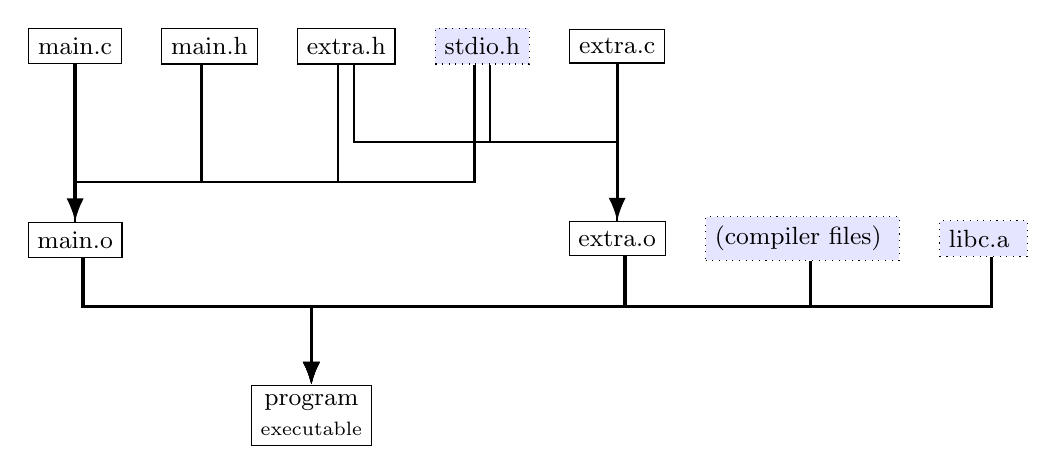
\begin{tikzpicture}
\tikzset{
    file/.style={font=\small,draw,align=center},
    file C/.style={file},
    file H/.style={file},
    file system/.style={file,dotted,fill=blue!10},
    file S/.style={file},
    file O/.style={file},
    produce main/.style={draw,very thick,-Latex},
    produce minor/.style={draw,thick},
}
\begin{scope}[every node/.style={on chain},start chain=going right,node distance=.5cm]
\node[file C] (main c) {main.c};
\node[file H] (main h) {main.h};
\node[file H] (extra h) {extra.h};
\node[file system] (stdio h) {stdio.h};
\node[file C] (extra c){extra.c};
\end{scope}
\node[file O,anchor=north] (main o) at ([yshift=-2cm]main c.south) {main.o};
\draw[produce main] (main c) -- (main o);
\foreach \nm in {main h,extra h,stdio h} {
    \draw[produce minor] ([xshift=-1mm]\nm.south) |- ([yshift=.5cm]main o.north) -- (main o.north);
}
\node[file O,anchor=north] (extra o) at ([yshift=-2cm]extra c.south) {extra.o};
\draw[produce main] (extra c) -- (extra o);
\foreach \nm in {extra h,stdio h} {
    \draw[produce minor] ([xshift=1mm]\nm.south) |- ([yshift=1cm]extra o.north) -- (extra o.north);
}
\node[file] (program) at ([xshift=3cm,yshift=-2cm]main o.south) { program \\ \scriptsize executable };
\node[anchor=west, file system] (compiler o) at ([xshift=.5cm]extra o.east) { (compiler files) };
\node[file system,anchor=west] (libc a) at ([xshift=.5cm]compiler o.east) {
    libc.a
};
\foreach \nm in {main o,extra o,compiler o,libc a} {
    \draw[produce main] ([xshift=1mm]\nm.south) |- ([yshift=1cm]program.north) -- (program.north);
}
% FIXME: show combining more files
\end{tikzpicture}
\end{frame}

\begin{frame}\frametitle{file extensions}
\begin{tabular}{ll|l}
name & ~ & \\\hline
    {\tt .c} & & C source code \\[1ex]
    {\tt .h} & & C header file  \\[1ex]
    {\tt .s} & (or {\tt .asm}) & assembly file \\[1ex]
    {\tt .o} & (or {\tt .obj}) & object file (binary of assembly) \\[1ex]
    (none) & (or {\tt .exe}) & executable file \\[1ex]
.a & (or {\tt .lib}) & statically linked library \\
    ~ & ~ & [collection of .o files] \\[1ex]
.so & (or {\tt .dll} or {\tt .dylib}) & dynamically linked library \\
    ~ & ~ & [`shared object'] \\
\end{tabular}
\end{frame}
